\documentclass[14pt,a4paper]{scrartcl}
\usepackage[left=25mm, right=20mm, top=20mm, bottom=30mm]{geometry}
\usepackage[utf8]{inputenc}
\usepackage[english,russian]{babel}
\usepackage[T1]{fontenc}
\usepackage{times}
\usepackage{listings}
\usepackage[usenames,dvipsnames]{color}
\usepackage{enumitem}
\usepackage{graphicx}
\usepackage{tikz}
\usepackage{scrextend}
\usepackage{ragged2e}
\usepackage{microtype}
\usepackage{indentfirst}

\justifying
\sloppy
\linespread{1,5}
\tolerance=500
\hyphenpenalty=10000
\emergencystretch=3em

\usetikzlibrary{trees,calc}
\usetikzlibrary{positioning}
\graphicspath{ {images/} }

\lstdefinelanguage{Dockerfile}{morekeywords={FROM, RUN, CMD, LABEL, MAINTAINER, EXPOSE, ENV, ADD, COPY, ENTRYPOINT, VOLUME, USER, WORKDIR, ARG, ONBUILD, STOPSIGNAL, HEALTHCHECK, SHELL}, morecomment=[l]{\#}, morestring=[b]"}

\lstset{language=R, basicstyle=\ttfamily, numbers=left, numberstyle=\color{Blue}, stepnumber=1, numbersep=5pt, backgroundcolor=\color{white}, showspaces=false, showstringspaces=false, showtabs=false, frame=single, rulecolor=\color{black}, tabsize=4, captionpos=b, breaklines=true, breakatwhitespace=false, keywordstyle=\color{RoyalBlue}, commentstyle=\color{YellowGreen}, stringstyle=\color{ForestGreen}}

\makeatletter
\newcount\dirtree@lvl
\newcount\dirtree@plvl
\newcount\dirtree@clvl
\def\dirtree@growth{%
  \ifnum\tikznumberofcurrentchild=1\relax
  \global\advance\dirtree@plvl by 1
  \expandafter\xdef\csname dirtree@p@\the\dirtree@plvl\endcsname{\the\dirtree@lvl}
  \fi
  \global\advance\dirtree@lvl by 1\relax
  \dirtree@clvl=\dirtree@lvl
  \advance\dirtree@clvl by -\csname dirtree@p@\the\dirtree@plvl\endcsname
  \pgf@xa=7mm\relax
  \pgf@ya=-13mm\relax
  \pgf@ya=\dirtree@clvl\pgf@ya
  \pgftransformshift{\pgfqpoint{\the\pgf@xa}{\the\pgf@ya}}%
  \ifnum\tikznumberofcurrentchild=\tikznumberofchildren
  \global\advance\dirtree@plvl by -1
  \fi
}

\tikzset{
  dirtree/.style={
    growth function=\dirtree@growth,
    every node/.style={anchor=north},
    every child node/.style={anchor=west},
    edge from parent path={(\tikzparentnode\tikzparentanchor) |- (\tikzchildnode\tikzchildanchor)}
  }
}
\makeatother

\begin{document}
    % Титульник
    \begin{titlepage}
        \begin{center}
            \large
            МИНИСТЕРСТВО ОБРАЗОВАНИЯ И НАУКИ\\
            РОССИЙСКОЙ ФЕДЕРАЦИИ\\
            \textbf{Федеральное агентство по образованию\\}
            \vspace{0.5cm}
            ТВЕРСКОЙ ГОСУДАРСТВЕННЫЙ УНИВЕРСИТЕТ\\
            \vspace{0.25cm}
            Факультет прикладной математики и информатики\\
            Кафедра математической статистики и системного анализа\\
            \vfill
            \textsc{ВЫПУСКНАЯ РАБОТА БАКАЛАВРА}\\[5mm]
            {\LARGE Разработка модуля непараметрического анализа данных в пакете R\\[2mm]}
            \bigskip
        \end{center}
        \vfill
        \hfill
        \begin{minipage}{0.4\textwidth}
            Автор:\\
            Семенков Филипп Андреевич\\
            \newline
            Научный руководитель:\\
            Сидорова Оксана Игоревна\\
        \end{minipage}
        \vfill
        \begin{center}
            Тверь, 2018 г.
        \end{center}
    \end{titlepage}

    % Оглавление
    \newpage
    \tableofcontents

    % Содержание
    % Теория
    \newpage
    \section{Теоретическая часть}
    \subsection{Введение}
    В учебном плане факультета прикладной математики и кибернетики на кафедре математической статистики и системного анализа мы изучаем довольно большое количество различных дисциплин.
    В курсе непараметрической статистики мы изучаем нормальное и экспоненциальное распределения, гамма - распределения, логарифмически нормальные и другие.
    Для решения задач непараметрической статистики используются методы, позволяющие изучать выборку небольшого объема с данными в которых содержатся такие параметры, о распределении которых мало известно или абсолютно ничего не известно.
    Такие методы не основаны на оценке параметров.

    \subsection{Практическая ценность}
    Для решения таких задач используются различные статистические пакеты, такие как пакет R.
    В пакете R существует большое количество библиотек, содержащих готовые функции, которые помогут решить задачу.

    Для вызова подобных функций, необходимо проделать несколько шагов:

    \begin{itemize}[noitemsep]
        \item Установка пакета R
        \item Поиск библиотеки с необходимой функцией
        \item Установка библиотеки
        \item Написание программы для вызова функции
    \end{itemize}

    Установить сам интерпретатор R довольно просто.
    К тому же для этого языка существуют IDE.
    Самый популярный из них это RStudio.
    RStudio в общем упрощает написание программы на языке R.
    Он включает в себя редактор кода, инструменты для отладки и визуализации.
    Найти и установить необходимую библиотеку не так просто.
    Необходимые функции разбросаны по разным пакетам.
    А некоторые пакеты имеют специфические зависимости, на установку и настройку которых может потребоваться много времени.
    Да и для написания программы необходимы знания языка и время на изучение пакетов.
    Всё это натолкнуло меня на мысль о создании универсального модуля в котором будут собраны необходимые пакеты.

    \subsection[Задел на будущее]{Задел на будущее}
    Просто собрать необходимые пакеты в одну программу это сложная задача, но ещё сложнее предоставить к нужным функциям единый удобный интерфейс, который можно будет использовать на различных устройствах.
    Для того, чтобы в любой момент можно было добавить или удалить функцию, поменять её описание и при этом не сломать всё остальное стоит разработать программный интерфейс приложения (API).
    API может помочь в наполнении программы функциями, а так же позволит использовать модуль не только в решении задач непараметрической статистики.
    В таком случае этот модуль будет полезен не только в рамках поставленной задачи.

    \subsection{Постановка задачи}
    \noindent Цель: Разработать модуль непараметрического анализа данных в пакете R.
	\noindent Задачи:
    \begin{enumerate}
        \item Разработать требования к программе
        \item Выбрать и изучить стек технологий, согласно требованиям
        \item Разработать структуру приложения
        \item Написать приложение
    \end{enumerate}

    \subsection{Требования к программе}
    Требования к поведению программы:
    \begin{itemize}
        \item Модуль должен являться приложением, написанным на языке R
        \item Модуль должен позволять решать задачи непараметрической статистики
        \item Модуль должен иметь пользовательский интерфейс
    \end{itemize}

    Требования к характеру поведения системы:
    \begin{itemize}
        \item Модуль должен иметь возможность расширения функционала
        \item Доступ к модулю может осуществляться с помощью различных устройств
        \item Устройства могут иметь различные операционные системы
        \item Пользовательский интерфейс должен корректно отображаться на устройствах с различными экранами
    \end{itemize}

    \subsection{Пользовательский интерфейс}
    Согласно требованиям к поведению программы, модуль должен иметь пользовательский интерфейс.
    Существует несколько видов пользовательских интерфесов.

    Основные виды пользовательских интерфесов:
    \begin{itemize}
        \item Консольный интерфейс
        \item Графический:
        \begin{itemize}
            \item Простой графический интерфейс
            \item WEB интерфейс
        \end{itemize}
    \end{itemize}

    Так как модуль должен являться приложением, написанным на языке R, то можно сделать ограничение написания интерфейса
    на языке R, чтобы не усложнять модуль различными языками программирования.
    Можно понять, что интерфейс должен отобразить решения задач непараметрической статистики.
    В таком случае следует учесть, что результатом может быть график.
    Также согласно требованиям к характеру поведения системы стоит учесть, что интерфейс должен корректно
    отображаться на различных устройствах с различными оперционными системами.

    Для того, чтобы определиться с видом пользовательского интерфейса, необходимо понять, какой из них лучше всго соответствует требованиям.
    При выборе консольного интерфейса могут возникнуть проблемы при отображении графиков, в таком случае нам больше подойдёт один из графических интерфейсов.
    Если мы выберем простое графическое (оконное) приложение, то в силу различных операционных систем могут возникнуть проблемы с переносом приложения.
    К тому же, по данным агентства 'We Are Social', возросло количество интернет-пользователей, большинство из них являются владельцами смартфонов\cite{Internet-statistic-2018}.
    Из этого всего следует, что приложение должно предоставлять web интерфейс.

    \subsection[Программный интерфейс приложения]{Программный интерфейс приложения (API)}
    Программный интерфейс приложения должен предоставлять возможность внедрить необходимую функцию в модуль.
    Стоит определить как в конечном итоге будет выглядеть функция и какой программный интерфейс необходимо предоставить.
    С точки зрения программирования, функция - это подпрограмма, которая принимает параметры и возвращает некоторый результат.
    С точки зрения математики, функция - это алгоритм, который также принимает параметры и возвращает некоторый результат.
    Для того чтобы в модуле различать функции, необходимо им выдать уникальные идентификаторы (названия функций).
    Чтобы лучше понимать что делает алгоритм стоит добавить описание.

    В конечном итоге становится понятным, интерфейс будет ожидать от наших подпрограмм:
    \begin{itemize}
        \item Название функции
        \item Описание функции
        \item Алгоритм
        \item Типы, имена и значения входных данных
        \item Типы, имена и значения выходных данных
    \end{itemize}
    На выходе API должен собрать такие подпрограммы и предоставить пользовательский интерфейс.

    \subsection[Развёртывание приложения]{Развёртывание приложения}
    Веб-приложение — это приложение, логика которого распределена между клиентом и сервером (клиент-серверное приложение)\cite{Web-app-wiki}.
    Клиентская часть веб-приложения представляет собой графический интерфейс.
    Это то, что пользователь видит на странице.
    Этот интерфейс отображается в браузере.
    Пользователь в свою очередь взаимодействует с веб-приложением через браузер.
    Сервером называется компьютер, выделенный из группы персональных компьютеров для выполнения какой-либо задачи без непосредственного участия человека.\cite{Server}
    Выделяют также веб сервер. Это сервер содержащий программу или скрипт, который обрабатывает запросы пользователя (точнее, запросы браузера)\cite{Web-app-struct}

    Выбор технологии для разворачивания веб приложения на сервере будут рассмотрены в практической части.

    % Практика
    \newpage
    \section[Практическая часть]{Практическая часть}
    \subsection[Выбор технологий]{Выбор технологий}
    В рамках задачи, необходимо определить, с помощью каких инструментов будет:
    \begin{itemize}
        \item разворачиваться сервер
        \item обрабатываться html запросы
        \item генерироваться пользовательский интерфейс
    \end{itemize}

    Для того чтобы развернуть приложение существует несколько возможных решений.

    Решение "в лоб" это написание установочного скрипта, который установит всё, что необходимо и запустит приложение на сервере (скрипт может быть как простым bash (sh) скриптом, так и чем-то сложным, созданным с использованием специальных инструментов).
    Недостатки такого подхода — это неустойчивость к ошибкам и плохая переносимость.
    Насколько бы хорошо не был написан скрипт, он не сможет учесть все возможные варианты развития событий., что скорее всего приведёт к остановке исполнения скрипта с ошибкой.
    Но при этом, скрипт уже мог внести какие-либо изменения, которые сложно или невозможно 'откатить'.

    Чтобы не было таких проблем можно запустить приложение в облачном сервисе.
    На виртуальный сервер вручную установить всё что нужно.

%	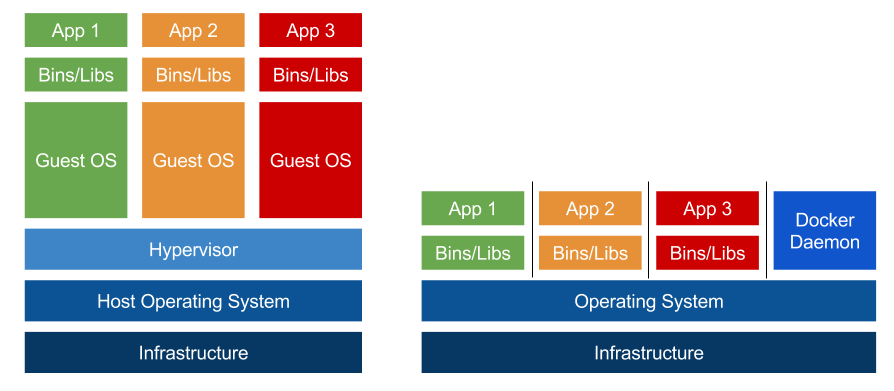
\includegraphics[width=\textwidth]{Docker-struct.png}


    \subsection[Развёртывание приложения]{Развёртывание приложения}
    \subsection[Алгоритм разворачивания сервера]{Алгоритм разворачивания сервера}
    \subsection[Алгоритм запуска приложения]{Алгоритм запуска приложения}
    \subsection[Пользовательский интерфейс]{Пользовательский интерфейс}
    \subsection[Программный интерфейс приложения]{Программный интерфейс приложения (API)}

    \newpage
    \subsection[Cтруктура приложения]{Cтруктура приложения}
    В конечном итоге получаем следующую струтуру приложения:\\
	\newline
	\begin{tikzpicture}[dirtree]
        \node {npsw/}
            child { node {src/}
                child { node {modules}
                    child { node {module1/}
                        child { node {server1.R} }
                        child { node {ui1.R} }
                    }
                    child { node {module2/}
                        child { node {server2.R} }
                        child { node {ui2.R} }
                    }
                    child { node {.....} }
                }
                child { node {util}
                    child { node {utilFunction1.R} }
                    child { node {utilFunction2.R} }
                    child { node {.....} }
                }
                child { node {app.R} }
            }
            child { node {npsw} }
            child { node {Dockerfile} };
	\end{tikzpicture}
    \newline
    Где:
    \begin{itemize}
        \item \textbf{npsw/}  - директория приложения
        \item \textbf{npsw} - скрипт, запускающий приложение
        \item \textbf{Dockerfile} - скрипт, разворачивающий сервер
        \item \textbf{src/} - директория исходного кода приложения
        \item \textbf{app.R} - код, описывающий API
        \item \textbf{modules/} - директория, содержащая модули, соответствующие написанному API
        \item \textbf{module1/} - директория одного из модулей
        \item \textbf{server1.R} - файл, описывающий алгоритм модуля 'module1'
        \item \textbf{ui1.R} - функция, описывающая пользовательский интерфейс модуля 'module1'
        \item \textbf{util/} - директория, содержащая утилитарные функции
        \item \textbf{utilFunction1.R} - файл, описывающий утилитарную функцию
    \end{itemize}

    % Примеры
    \newpage
    \section[Примеры решения задач]{Примеры решения задач}
%    \subsection[Какя-то задача]{Какя-то задача}

    % Заключение
    \newpage
    \section[Заключение]{Заключение}

    % Список литературы
    \newpage
    \addcontentsline{toc}{section}{Список литературы}
    \begin{thebibliography}{9}
        \bibitem{Internet-statistic-2018}Social media use jumps in Q1 despite privacy fears
        \newblock --- https://wearesocial.com/uk/blog/2018/04/social-media-use-jumps-in-q1-despite-privacy-fears

        \bibitem{Web-app-wiki}Веб-приложение
        \newblock --- https://ru.wikipedia.org/wiki/Веб-приложение

        \bibitem{Server}Сервер (аппаратное обеспечение)
        \newblock --- https://ru.wikipedia.org/wiki/Сервер

        \bibitem{Web-app-struct}Структура веб-приложения
        \newblock --- http://labaka.ru/likbez/struktura-veb-prilozheniya

        \bibitem{Docker-habra}Docker. Зачем и как
        \newblock --- https://habr.com/post/309556

    \end{thebibliography}
\end{document}

% Исходный код R
%\newpage
%\section{Исходный код R}
%\begin{lstlisting}[language=R]
%library(foreign)
%foo <- rnorm(100)
%# writing a function
%bar <- apply(
%foo, 1, function(x){
%y <- sqrt(x)
%cat(
%paste('The result is ', x )
%)
%}
%)
%bar
%str(bar)
%foo + bar
%\end{lstlisting}

%https://ru.sharelatex.com/learn/Inserting_Images

%\begin{tikzpicture}[>=stealth,every node/.style={shape=rectangle,draw,rounded corners},]
%    % create the nodes
%    \node (c1) {Chapter 1};
%    \node (c4) [below right=of c1]{Chapter 4};
%    \node (c5) [below left=of c4]{Chapter 5};
%    \node (c6) [right =of c5]{Chapter 6};
%    \node (c7) [right =of c6]{Chapter 7};
%    \node (c8) [right =of c7]{Chapter 8};
%    \node (c9) [right =of c8]{Chapter 9};
%    \node (c2) [below =of c5]{Chapter 2};
%    \node (c3) [below right =of c2]{Chapter 3};
    % connect the nodes
%    \draw[->] (c1) to[out=0,in=135] (c4);
%    \draw[->] (c1.west) to[out=180,in=180] (c2.west);
%    \draw[->] (c4) to[out=180,in=75] (c5);
%    \draw[->] (c4) -- (c6);
%    \draw[->] (c4.south east) -- (c7);
%    \draw[->] (c4.east) to[out=0,in=110] (c8);
%    \draw[->] (c4.east) to[out=0,in=110] (c9);
%    \draw[->,dashed] (c2) -- (c5);
%    \draw[->,dashed] (c2) -- (c6);
%    \draw[->,dashed] (c2) -- (c7.south);
%    \draw[->,dashed] (c2) -- (c8.south);
%    \draw[->] (c2) -- (c3);
%\end{tikzpicture}
